\subsection{Disparity Algorithm}
Some important properties of the stereo camera setup used in this project were taken advantage of in order to extract 3D depth information from 2D image data. Since both cameras captured imagery of the same scene from slightly different vantage points, depth information on the scene was extracted by calculating the pixel offsets, or disparity, between the same object's relative location in each image. Given this pixel offset, the distance from the camera pair to a given object was determined using simple geometry based on the focal length and baseline of the stereo camera pair. Each camera needed to have the same focal length, or distance from the image sensor to the lens of the camera. The baseline, or distance between image sensors of the stereo camera pair was equivalent to 63mm. Note that this number was chosen to reflect the average distance between a pair of human eyes \cite{collins}. 
\subsubsection{Image Rectification} \label{rectsec}
One simple method for determining the disparity between objects in a stereo image pair is known as the Sum of Absolute Differences. The Sum of Absolute Differences algorithm operates under the assumption that objects in both camera images lie on the same horizontal line between both images, known as an epipolar line \cite{collins}. An example of shared epipolar lines between camera imagery is shown in Figure \ref{epipolarLines} below. Although an ideal stereo camera setup contains shared epipolar lines between camera images, raw image data from seemingly identical cameras will contain slight differences in object location based on the physical position of the camera modules, as well as minor differences in the lenses of each camera. Both input images are normally adjusted to share the same epipolar lines through a post-processing step known as image rectification \cite{collins}. 
\par
\begin{figure}[H]
	\centerline{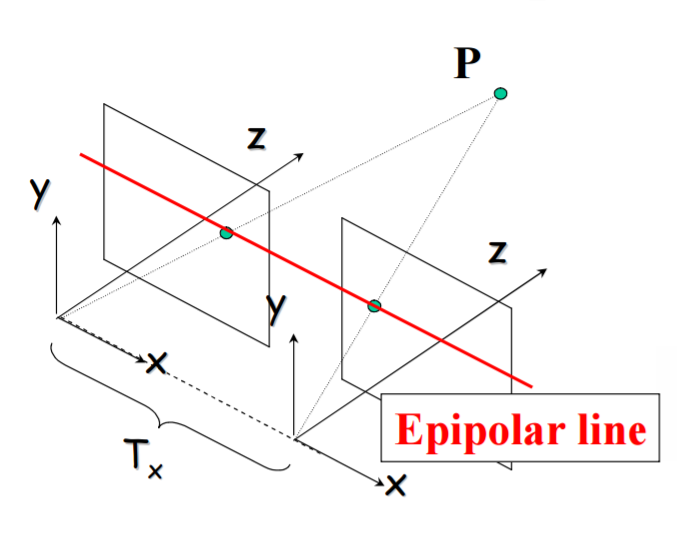
\includegraphics[width=0.5\textwidth]{epipolarLines.PNG}}
	\caption{Horizontal Epipolar Lines \cite{collins}}
	\label{epipolarLines}
\end{figure}
\par
A pictorial representation of the process of stereo image rectification is shown in Figure \ref{rectification} below \cite{mattoccia_slides}. This specific rectification example was achieved using a 3x3 matrix coordinate transform based on parameters obtained from the external calibration process. 
\begin{figure}[H]
	\centerline{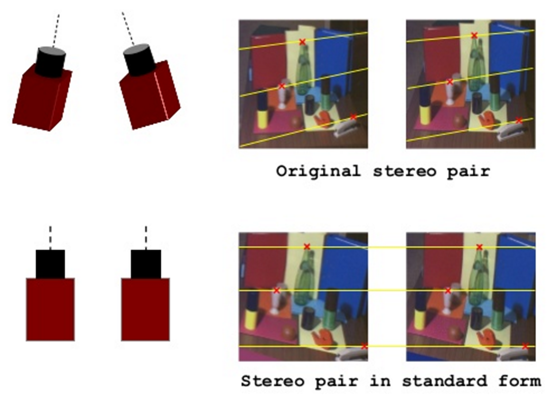
\includegraphics[width=0.5\textwidth]{rectification.png}}
	\caption{Stereo Image Rectification \cite{mattoccia_slides}}
	\label{rectification}
\end{figure}
\par
After a given pair of images has been rectified, it is then possible to perform the Sum of Absolute Differences on the given image pair in order to extract depth information. 
\subsubsection{Sum of Absolute Differences} \label{SADexample}
The method used in our disparity algorithm implementation was known as the Sum of Absolute Differences, or SAD. SAD is a common digital image processing technique used to measure the similarity between blocks of image data. In the case of our stereo camera interface, a SAD algorithm was used to search along epioplar lines in the right image for pixel blocks that matched a template block selected from the left camera image. This process was performed using 7x7 pixel search blocks over 20 pixel horizontal ranges, and was repeated throughout the image. The expression for the sum of absolute differences is shown in Equation \ref{disparityEQN} below. 
\par
% sum(sum(abs(template-block)))
\begin{equation}\label{disparityEQN}
SAD = \sum_{x}^{}\sum_{y}^{}|template-block|
\end{equation}
\par
A visual representation of the Sum of Absolute differences is shown in Figure \ref{SAD}, with the top image showing the left image template block, and the middle image showing the right image search window in relation to the location of the template block. Below both images is a visual representation of the Sum of Absolute Differences between the template block and the current search block, outlined in white. In the case of the given example, the template and search blocks are relatively different, resulting in a high SAD value. 
\par
\begin{figure}[h]
	\centerline{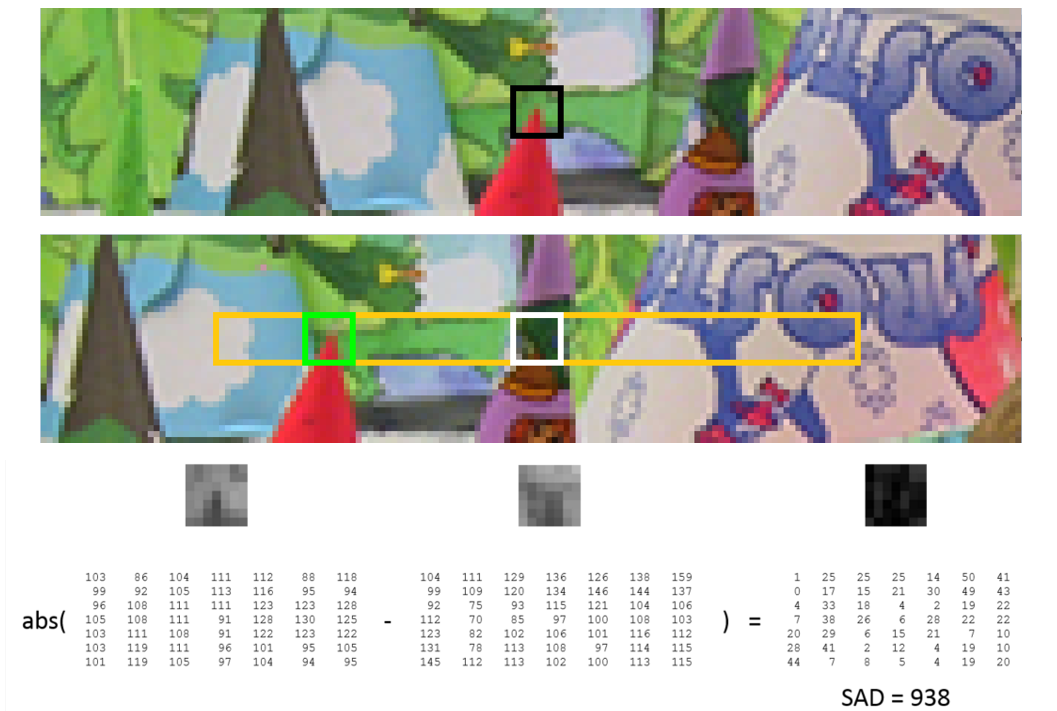
\includegraphics[width=0.75\textwidth]{SAD.PNG}}
	\caption{Sum of Absolute Differences \cite{mccormick}}
	\label{SAD}
\end{figure}
\par
Since the disparity algorithm used in this implementation calculated the sum of absolute differences for multiple search blocks, the resulting SAD values for each search block were then compared to find the location of the most similar matching block in the search image. Due to the nature of the SAD algorithm, lower SAD values indicated higher similarity between the template and search blocks. This comparison is demonstrated in Figure \ref{blockMatching} below. In the case of Figure 
\ref{blockMatching}, higher match score values for each search block indicate lower SAD values.
\par
\begin{figure}[h]
	\centerline{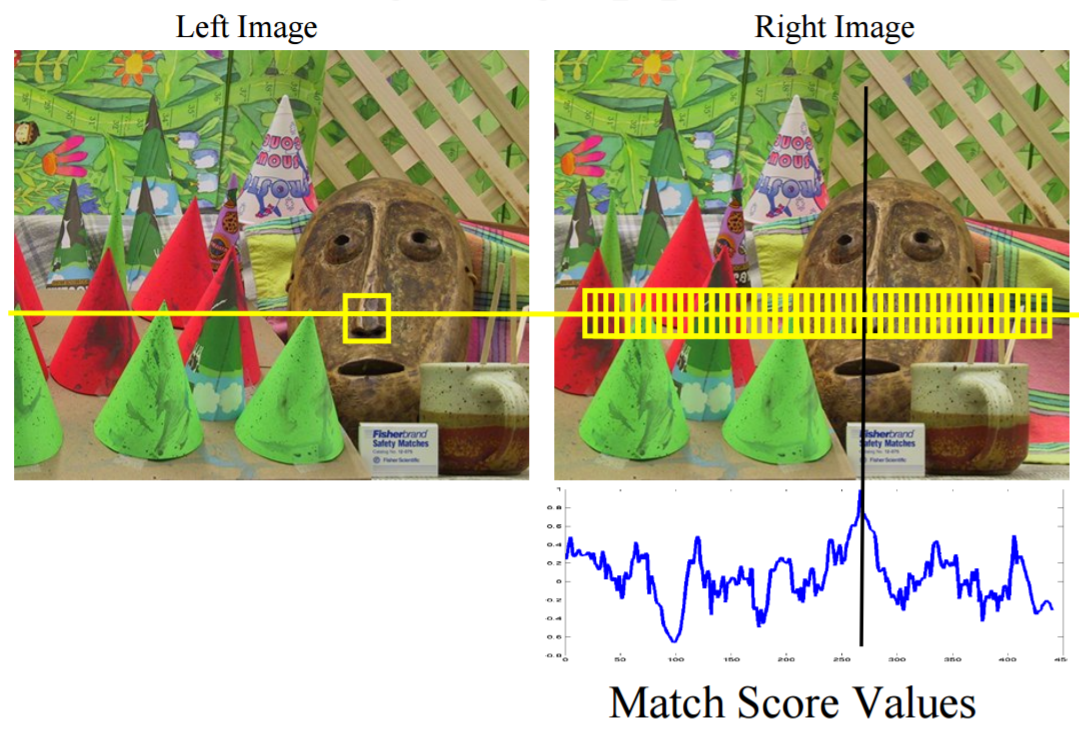
\includegraphics[width=0.75\textwidth]{blockMatching.PNG}}
	\caption{Block Matching Overview \cite{collins}}
	\label{blockMatching}
\end{figure}
\par
In the project implementation, the SAD at multiple search points was used to estimate the pixel offset between the template block and matching search block based on array index locations, since all SAD values for a single search were stored in a vector. This pixel offset was equivalent to the disparity value for a given template and search block. The disparity $d$ at a given point was then transformed into a unit of distance using the focal point $f$ and baseline distance $T_x$ between image sensors as shown in Equation \ref{disp2dist} below. 
\par
\begin{equation}\label{disp2dist}
depth = Z = \frac{fT_x}{d}
\end{equation}
\par
Pixel coloration values in a disparity image were based on the distance calculation shown in Equation \ref{disp2dist}, where each pixel was referenced to the disparity at a given template block's location. As an example, a disparity image created from a given pair of test images is shown in Figure \ref{disparityOutput} below. 
\par
\begin{figure}[H]
	\centerline{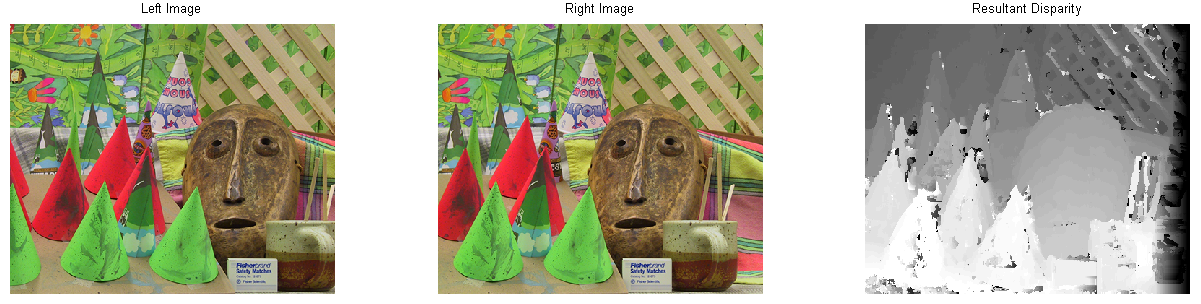
\includegraphics[width=1.1\textwidth]{disparity.png}}
	\caption{Disparity Algorithm Output}
	\label{disparityOutput}
\end{figure}